\documentclass[12pt,a4paper,oneside]{article}
\usepackage[utf8]{inputenc}
\usepackage{t1enc} % hyphenate accented chars
\usepackage[hungarian]{babel}
\usepackage{../fedlap}
\usepackage{fancyhdr} % elofej, elolab
\usepackage{graphicx}
\usepackage{datetime} % specify date format
\setcounter{secnumdepth}{3} % enable subsubsection

% hasonlitson a doc verziora
\addtolength{\voffset}{-1cm}

% cim
\csapat{nand}{39}
\konzulens{Bozóki Szilárd}
\datum{\todaynum}

% csapattagok
\taga{Berki Endre}{HQNHER}{berkiendre@gmail.com}
\tagb{Fodor Bertalan Ferenc}{H4T1UX}{foberci@gmail.com}
\tagc{Kádár András}{JFENWR}{arycika@gmail.com}
\tagd{Thaler Benedek}{EDDO10}{thalerbenedek@gmail.com}

\setlength{\headheight}{1.3em}
\setlength{\headsep}{2em}

% elofej, elolab
\fancyhf{}

\fancyhead[OL] { \tiny \leftmark{} }
\fancyhead[OR] { \tmpcsapat }

\fancyfoot[OR] { \thepage }
\fancyfoot[OL] { \tmpdatum }

\pagestyle{fancy}

% custom date format, according to customer request
% you have to use the \todaynum command instead of today,
% becouse babel overrides it, and I couldn't find a way to override
% it again. I was tempted to call this format \todaybozoki
\newcommand{\todaynum}{\the\year. \twodigit\month. \twodigit\day}


\usepackage{enumitem}
\usepackage{textcomp}
\usepackage[utf8]{inputenc}
\usepackage[T1]{fontenc}

\begin{document}

\anyag{11. Grafikus felület specifikációja}
\fedlap

\addtocounter{section}{10}
\section{Grafikus felület specifikációja}

	\subsection{A grafikus interfész}
	%A menürendszer, a kezelői felület grafikus képe. A grafikus  felület megjelenését, a használt ikonokat, stb screenshot-szer ű képekkel kell bemutatni. Az épít észetben ez a homlokzati terv.
	A grafikus felület megjelenítésére is az eredeti program felülete jelentett iránymutatást, egy kép az eredeti játékból:
	\begin{center}
		    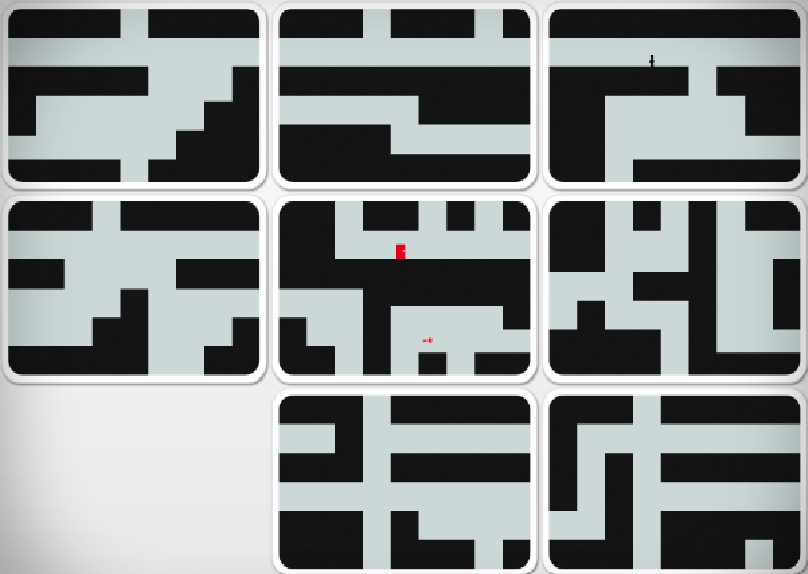
\includegraphics[scale=0.7]{resources/gui_original.png}
	  \end{center}
	
	A program felhasználói felületének tervezése során a felület kialakítását az egyszerűség és könnyen irányíthatóság irányelvei alakította ki. A menürendszer  felépítését az opciók minél gyorsabb elérésérére való törekvés határozta meg. Emiatt a játék közbeni lehetőségek mind elérhetőek egyetlen kattintással, vagy a megfelelő billentyű lenyomásával, gördülékenyebbé téve a játékmenetet. A fenti szempontok figyelembe vételével a felület látványterve:
	\begin{center}
		    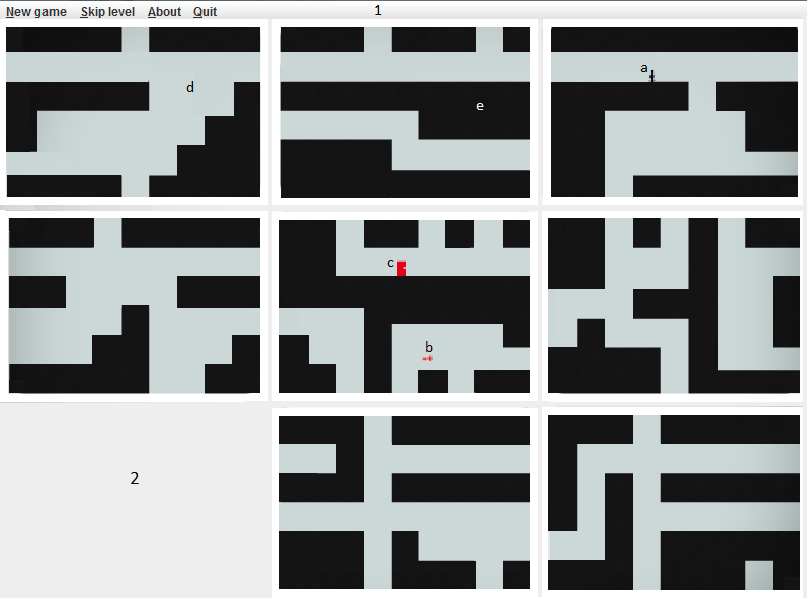
\includegraphics[scale=0.7]{resources/gui_own.png}
	 \end{center}
	 Az ábrán számokkal megjelölt kezelő-, és játékelemek:
	 \begin{description}	 
	  \item[1 Menüsáv] Az egyes opciók elérése.
 			\begin{description}
 			\item[1.1 New game]  Új játék kezdése.
 			\item[1.2 Skip level] A játék a következő pályára ugrik.
 			\item[1.3 About] A játék készítésével kapcsolatos információk érhetőek el.
 			\item[1.4 Quit] A játékból való kilépés.
			\end{description}
 	  \item[2 Játéktér] A folyamatban levő játék megjelenítése.
 	  \item[3 Stickmanek] A játékos által irányítható stickmanek.
 	  \item[4 Kulcs] Az ajtó nyitásához szükséges kulcs.
 	  \item[5 Ajtó] A pályáról való továbblépéshez szükséges kijárat.
 	  \item[6 Üres terület] A stickmanek által bejárható terület.
 	  \item[7 Fal] Járhatatlan szakasz.
     \end{description}

		\subsection{A grafikus rendszer architektúrája}
		%A felület m űködésének elve, a grafikus rendszer architektúrája (struktúra diagramok). A struktúra diagramokon a prototípus azon és cs ak azon osztályainak  is szerepelnie kell, amelyekhez a grafikus felületet létrehozó osztályok kapcsolódnak.
		
		\subsubsection{A felület működési elve}
		%Le kell írni, hogy a grafikai megjelenésért felelős osztályok, objektumok hogyan kapcsolódnak a meglevő rendszerhez, a megjelenítés során mi volt az alapelv. Törekedni kell az MVC megvalósításra. Alapelvek lehetnek: push  alapú: a modell értesíti a felületet, hogy változott; pull  alapú: a felület kérdezi le a modellt, hogy változott-e;  kevert: a kett ő kombinációja.
		A grafikus felület a \texttt{Game} osztály által szolgáltatott publish/subscribe mintát megvalósító kommunikációs csatornán keresztül értesül a modell változásairól. A felület továbbá ismeri az aktuális \texttt{Game} objektumot, így téve lehetővé a játék állapotának megjelenítését. Amikor a modell megváltozik, ezen a csatornán egy \texttt{invalidate} esemény érkezik, melynek hatására a megjelenésért felelős osztályok újrarajzolják a grafikus felületet. Az újrarajzolás során a grafikus felület kérdezi le a \texttt{Game} osztály állapotát (melybe beleértendő az aktuális pálya állapota és a nézet), ami alapján a rajzolást végzi.
		
		\subsubsection{A felület osztály-struktúrája}
		%Osztálydiagram. Minden új osztály, és  azon régiek, akik az újakhoz közvetlenül kapcsolódnak.
			
	    \begin{center}
		    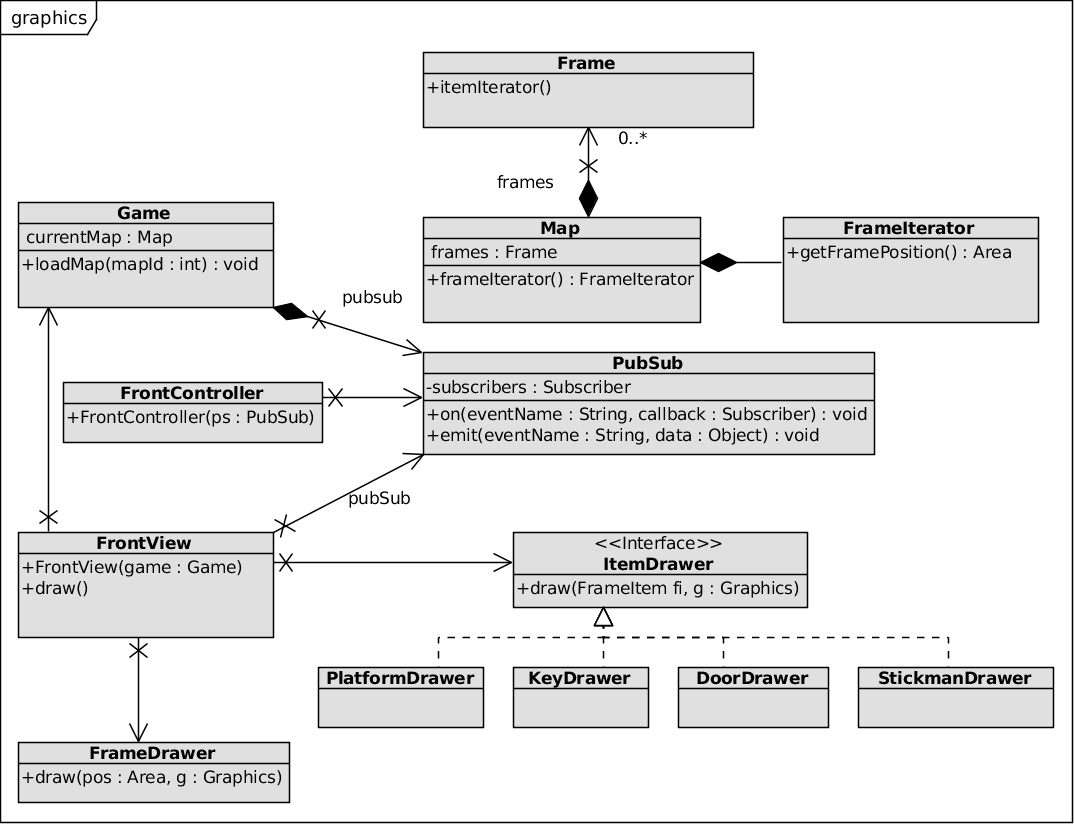
\includegraphics[scale=0.88]{resources/graphics.png}
	    \end{center}

	\subsection{A grafikus objektumok felsorolása}
	%Az új osztályok felsorolása. Az  régi osztályok közül azoknak a  felsorolása, ahol változás volt. Ezek esetén csak a változásokat kell leírni.	
	
	%GENERATOR:CLASS_DESCRIPTIONS
		\subsubsection{DoorDrawer}
			\begin{description}

				\item[Felelősség] Ajtókat rajzol ki.

				\item[Ősosztályok] (nincs)
				\item[Interfészek] ItemDrawer.
				\item[Attribútumok] (nincs)
				\item[Metódusok]$\ $
					\begin{description}
						\item[\texttt{+draw(fi : FrameItem, g : Graphics)}] \hfill \\Kirajzolja az átadott ajtót az átadott Graphics objektumon. 
					\end{description}
			\end{description}

		\subsubsection{Frame}
			Kibővített osztály.
			\begin{description}
				\item[Metódusok]$\ $
					\begin{description}
						\item[\texttt{+itemIterator() : Iterator}] \hfill \\Visszaad egy iteratort, mely a tartalmazott  elemeken megy végig. 
					\end{description}
			\end{description}
			
		\subsubsection{FrameDrawer}
			\begin{description}

				\item[Felelősség] Kereteket rajzol ki.

				\item[Ősosztályok] (nincs)
				\item[Interfészek] (nincs)
				\item[Attribútumok] (nincs)
				\item[Metódusok]$\ $
					\begin{description}
						\item[\texttt{+draw(f : Frame, g : Graphics)}] \hfill \\Kirajzol egy keretet 
					\end{description}
			\end{description}

		\subsubsection{FrontController}
			\begin{description}

				\item[Felelősség] Felhasználói parancsok fogadása, értelemezése, továbbítása.

				\item[Ősosztályok] (nincs)
				\item[Interfészek] (nincs)
				\item[Attribútumok]$\ $
					\begin{description}
						\item[\texttt{-pubSub : PubSub}]Kommunikációs csatorna a Game felé.
					\end{description}
				\item[Metódusok] (nincs)
			\end{description}
			
		\subsubsection{FrontView}
			\begin{description}

				\item[Felelősség] Kirajzolja a pálya aktuális állapotát, a benne lévő keretekkel, elemekkel stb. együtt, valamint megjeleníti a vezérlőket (pl. következő pályára lépés).

				\item[Ősosztályok] (nincs)
				\item[Interfészek] (nincs)
				\item[Attribútumok]$\ $
					\begin{description}
						\item[\texttt{-canvas : JPanel}]Az aktuális pálya megjelenítésére szolgáló terület.
						\item[\texttt{-drawers : Map}]A különböző típusú FrameItemekhez tartozó rajzoló osztályok tárolója.
						\item[\texttt{-game : Game}]A játék modellje
					\end{description}
				\item[Metódusok]$\ $
					\begin{description}
						\item[\texttt{-draw(g : Graphics)}] \hfill \\Gondoskodik a keretek és keret elemek canvaszra történő kirajzolásáról. 
						\item[\texttt{-initGUI()}] \hfill \\Inicializálja a grafikus interfészt,  többek közt megjeleníti a játékhoz tartozó ablakot. 
						\item[\texttt{-repaint()}] \hfill \\Újrarajzolja az aktuális pályát. 
					\end{description}
			\end{description}

		\subsubsection{ItemDrawer} Interfész.
			\begin{description}

				\item[Felelősség] FrameItemeteket rajzol ki.

				\item[Ősosztályok] (nincs)
				\item[Metódusok]$\ $
					\begin{description}
						\item[\texttt{+draw(fi : FrameItem, g : Graphics)}] \hfill \\Kirajzolja az átadott FrameItemet az átadott Graphics objektumon. 
					\end{description}
			\end{description}

		\subsubsection{KeyDrawer}
			\begin{description}

				\item[Felelősség] Kulcsokat rajzol ki.

				\item[Ősosztályok] (nincs)
				\item[Interfészek] ItemDrawer.
				\item[Attribútumok] (nincs)
				\item[Metódusok]$\ $
					\begin{description}
						\item[\texttt{+draw(fi : FrameItem, g : Graphics)}] \hfill \\Kirajzolja az átadott kulcsot az átadott Graphics objektumon. 
					\end{description}
			\end{description}

		\subsubsection{Map}
			Kibővített osztály.
			\begin{description}
				\item[Metódusok]$\ $
					\begin{description}
						\item[\texttt{+frameIterator() : Map.FrameIterator}] \hfill \\Visszaad egy iteratort, mellyel a tartalmazott kereteken lehet végigmenni 
					\end{description}
			\end{description}

		\subsubsection{Map.FrameIterator}
			\begin{description}

				\item[Felelősség] A mögöttes implementációtól függetlenül felsorolja a pálya által tartalmazott kereteket.

				\item[Ősosztályok] (nincs)
				\item[Interfészek] Iterator.
				\item[Attribútumok]$\ $
					\begin{description}
						\item[\texttt{-currentColumnIterator : Iterator}]Aktuális oszlop iteratora
						\item[\texttt{-currentRowIndex : int}]Aktuális sor indexe
						\item[\texttt{-nextColumnIndex : int}]Következő oszlop indexe
					\end{description}
				\item[Metódusok]$\ $
					\begin{description}
						\item[\texttt{+getFramePosition() : Area}] \hfill \\Megadja az aktuális keret által elfoglalt  pozíciót a pálya keretrácsában.    A bal felső sarokban a x:0, y:0  pozíciójú keret található. 
						\item[\texttt{-getNextColumn() : List}] \hfill \\Váltás a következő oszlopra 
						\item[\texttt{+hasNext() : boolean}] \hfill \\Ellenőrzi, hogy van-e még bejáratlan keret 
						\item[\texttt{+next() : Frame}] \hfill \\Lépés a következő keretre 
					\end{description}
			\end{description}
			
		\subsubsection{PlatformDrawer}
			\begin{description}

				\item[Felelősség] Platformokat rajzol ki.

				\item[Ősosztályok] (nincs)
				\item[Interfészek] ItemDrawer.
				\item[Attribútumok] (nincs)
				\item[Metódusok]$\ $
					\begin{description}
						\item[\texttt{+draw(fi : FrameItem, g : Graphics)}] \hfill \\Kirajzolja az átadott platformot az átadott Graphics objektumon. 
					\end{description}
			\end{description}

		\subsubsection{StickmanDrawer}
			\begin{description}

				\item[Felelősség] Stickmaneket rajzol ki.

				\item[Ősosztályok] (nincs)
				\item[Interfészek] ItemDrawer.
				\item[Attribútumok] (nincs)
				\item[Metódusok]$\ $
					\begin{description}
						\item[\texttt{+draw(fi : FrameItem, g : Graphics)}] \hfill \\Kirajzolja az átadott stickmant az átadott Graphics objektumon. 
					\end{description}
			\end{description}
%GENERATOR:CLASS_DESCRIPTIONS

	\clearpage
	\subsection{Kapcsolat az alkalmazói rendszerrel}
	%Szekvencia-diagramokon ábrázolni kell a grafikus rendszer működését. Konzisztens kell legyen az el őz ő alfejezetekkel. Minden metódus,  ami ott szerepel, fel kell tűnjön valamelyik szekvenciában. Minden metódusnak, ami szekvenciában  szerepel, szereplnie kell a valamelyik osztálydiagramon.
		\subsubsection{Initialize}
		    \begin{center}
			    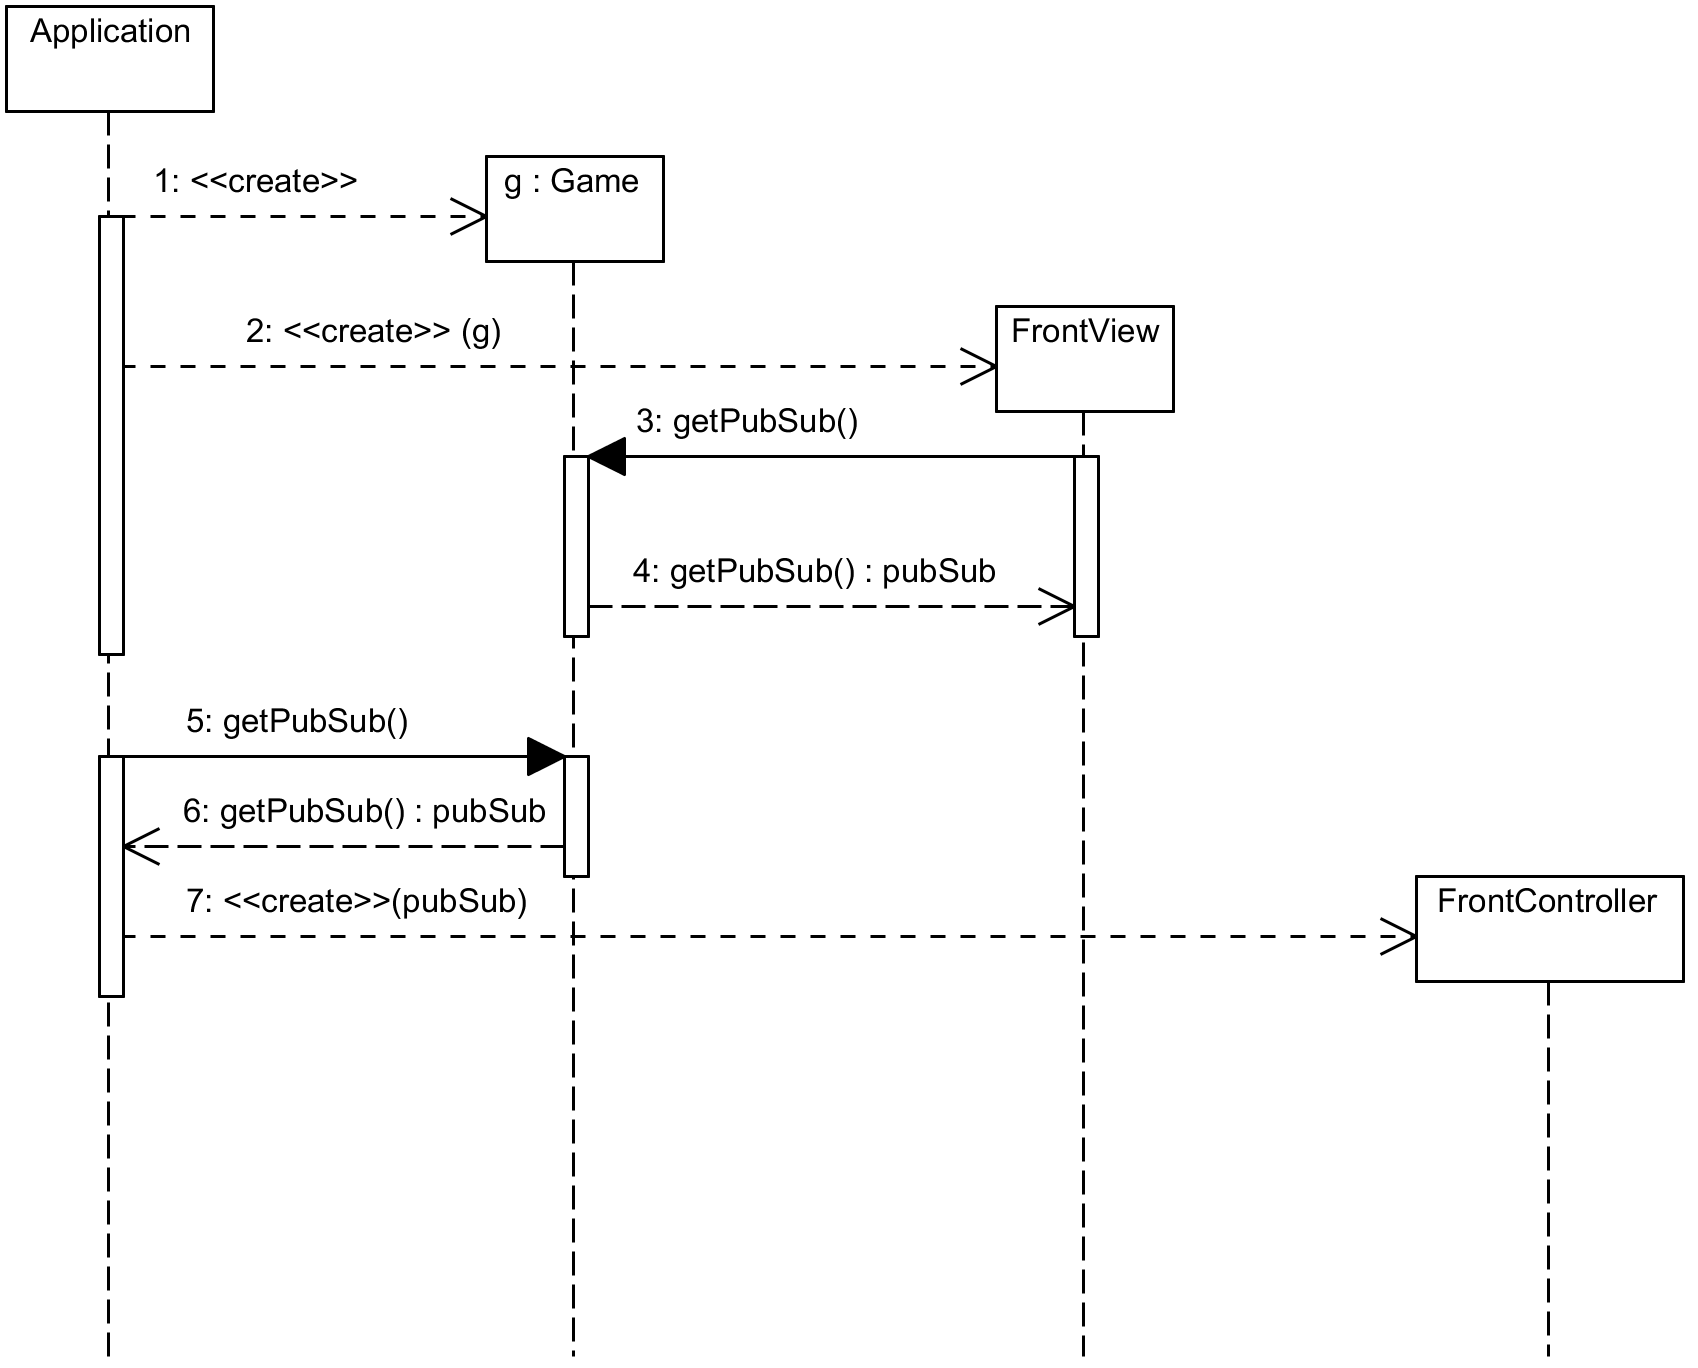
\includegraphics[scale=0.88]{resources/init.png}
		    \end{center}

		\subsubsection{Event}
		    \begin{center}
			    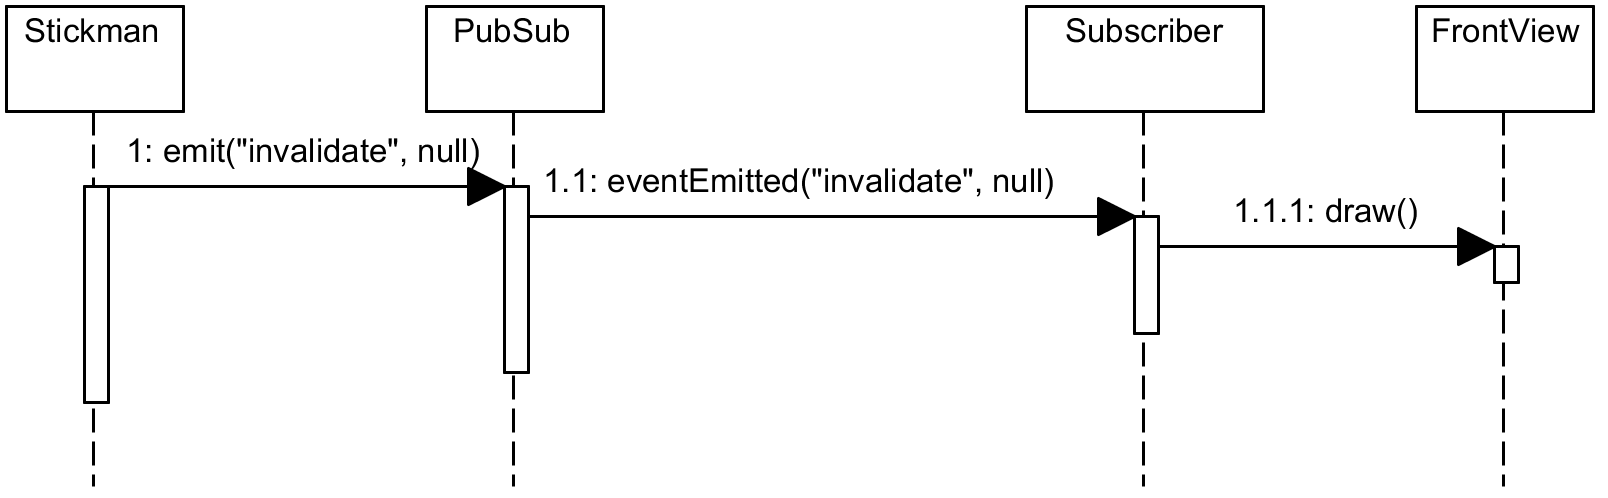
\includegraphics[scale=0.88]{resources/event.png}
		    \end{center}

		\subsubsection{Kirajzolás}
		    \begin{center}
			    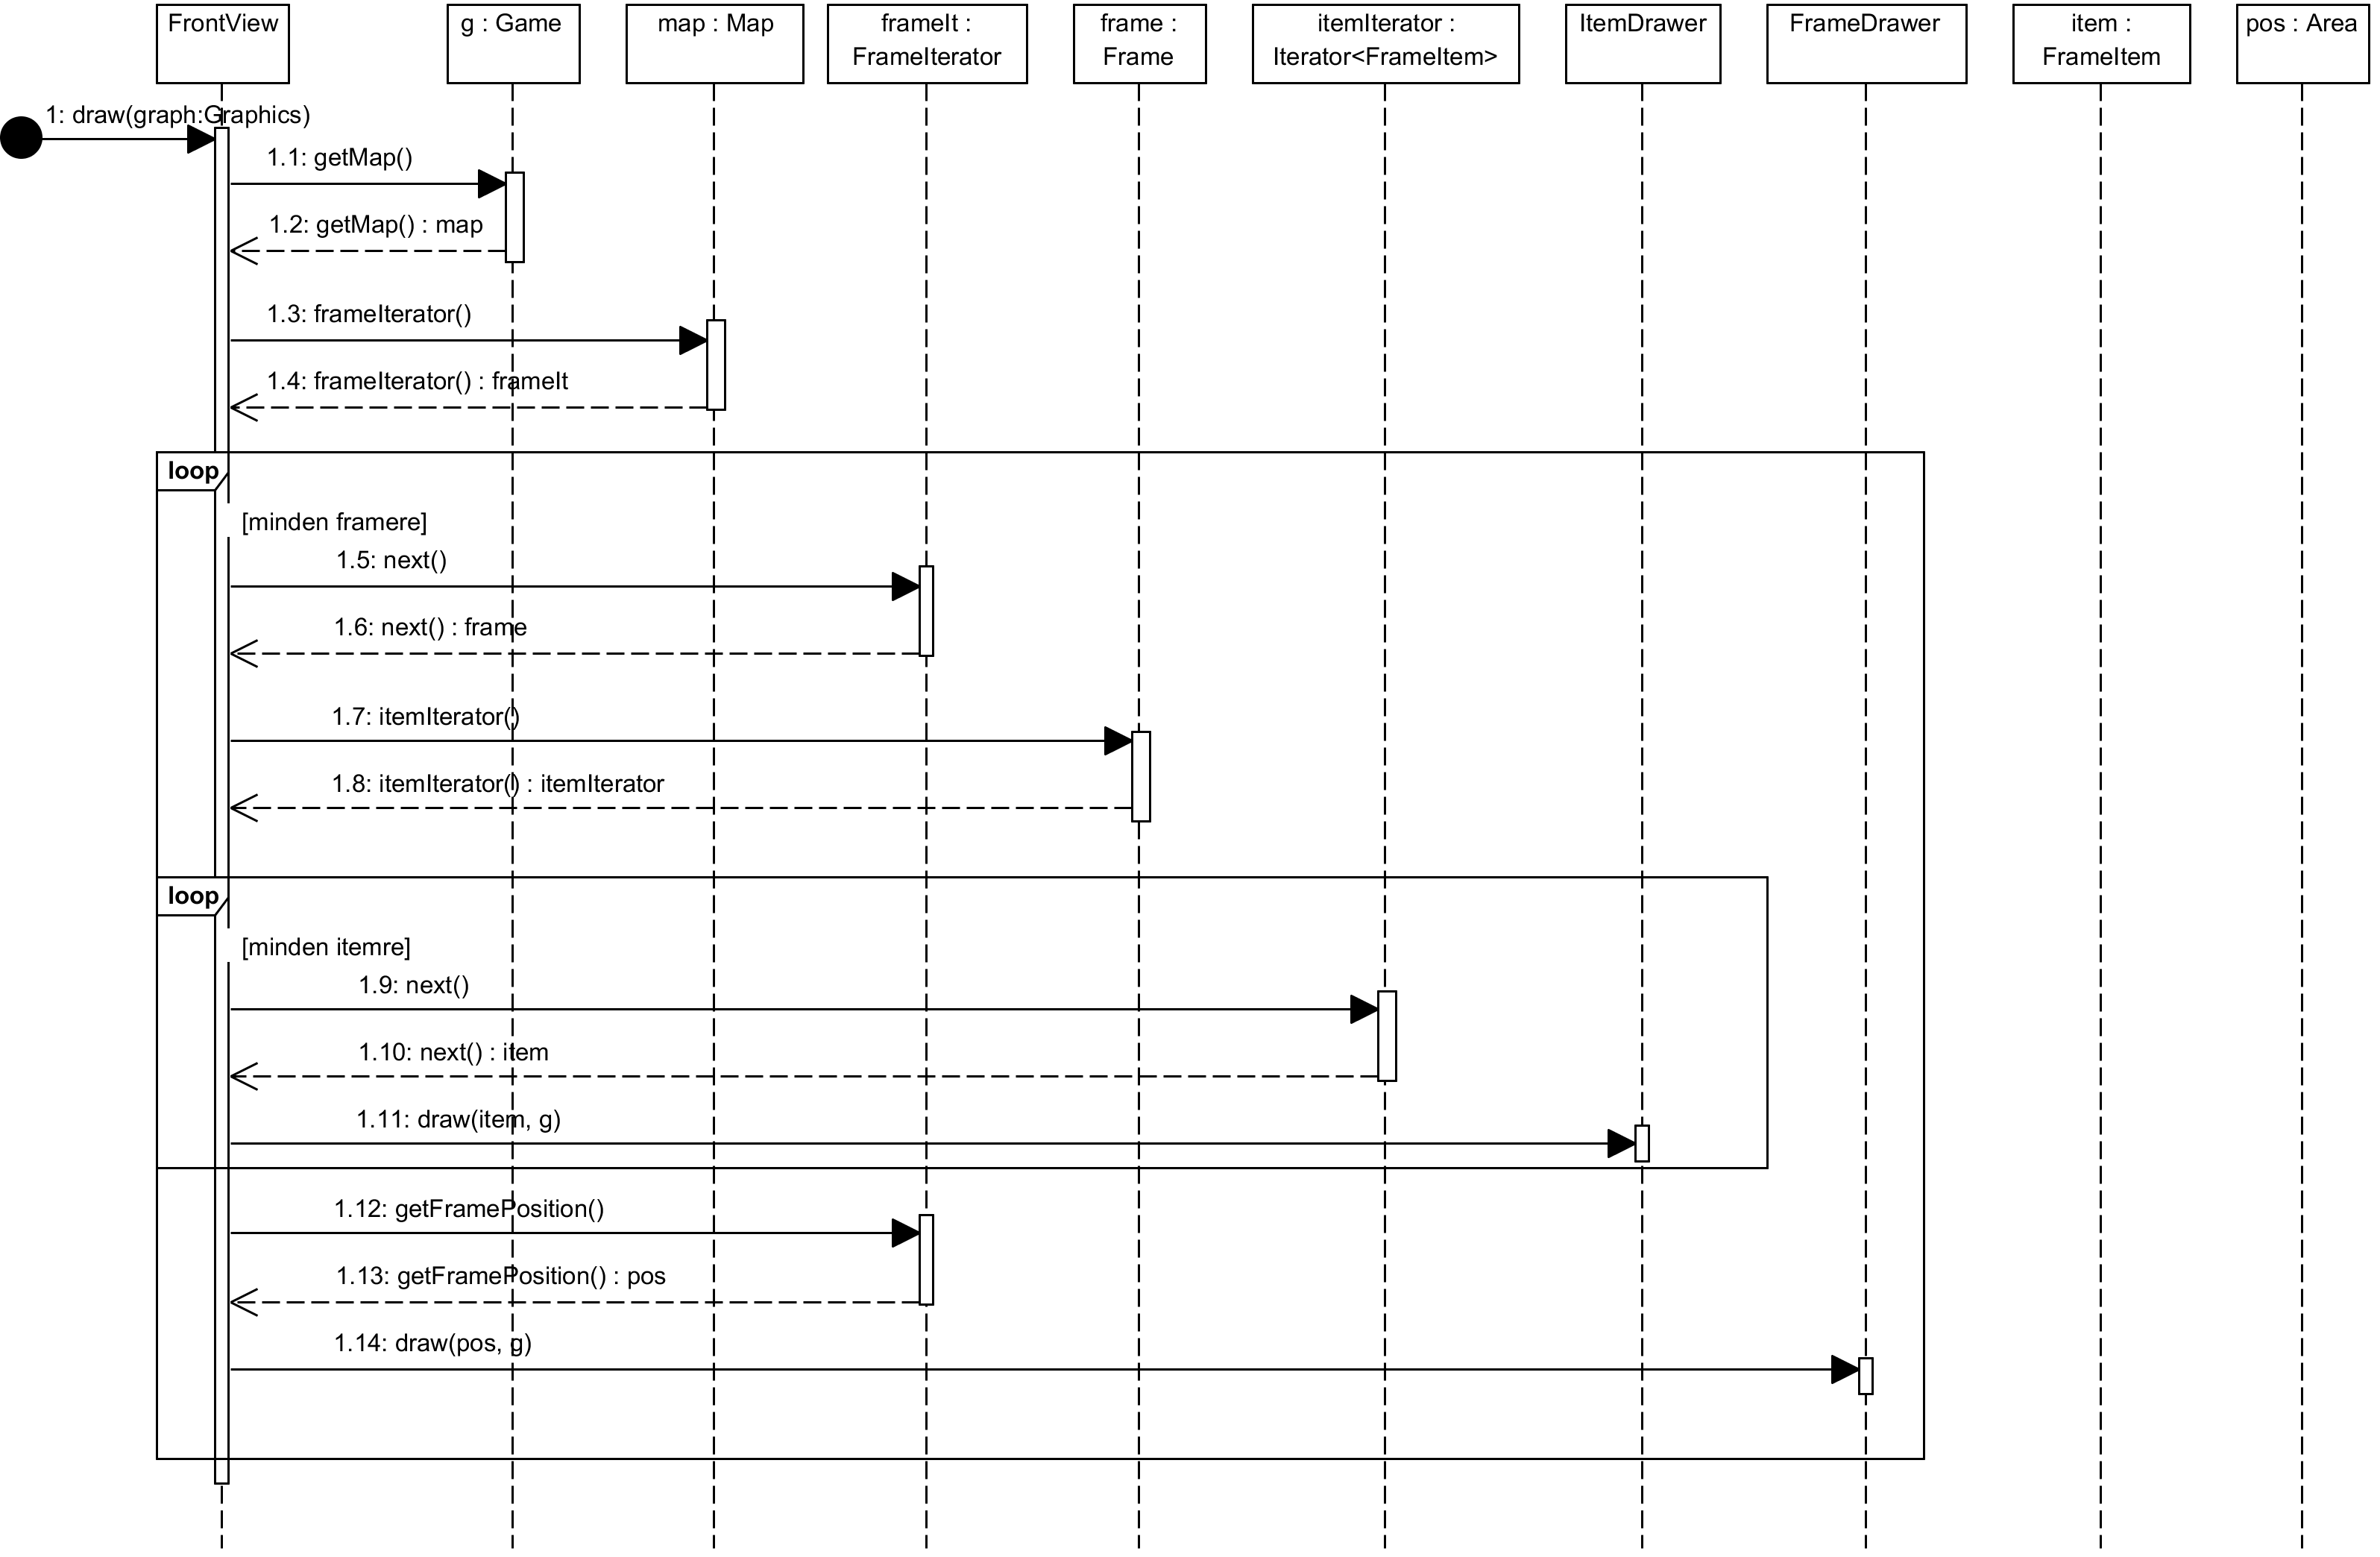
\includegraphics[scale=0.70, angle=-90]{resources/drawing.png}
		    \end{center}
	
		\subsection{Napló}
	% The diary generator uses the following comments to identify the beginning and the ending of the generated diary
	% The following content is auto generated, please do NOT modify, edit the related shared document instead.
	%GENERATOR:DIARY
	
	%GENERATOR:DIARY
\end{document}
